\setcounter{ExampleCounter}{1}
\marginnote{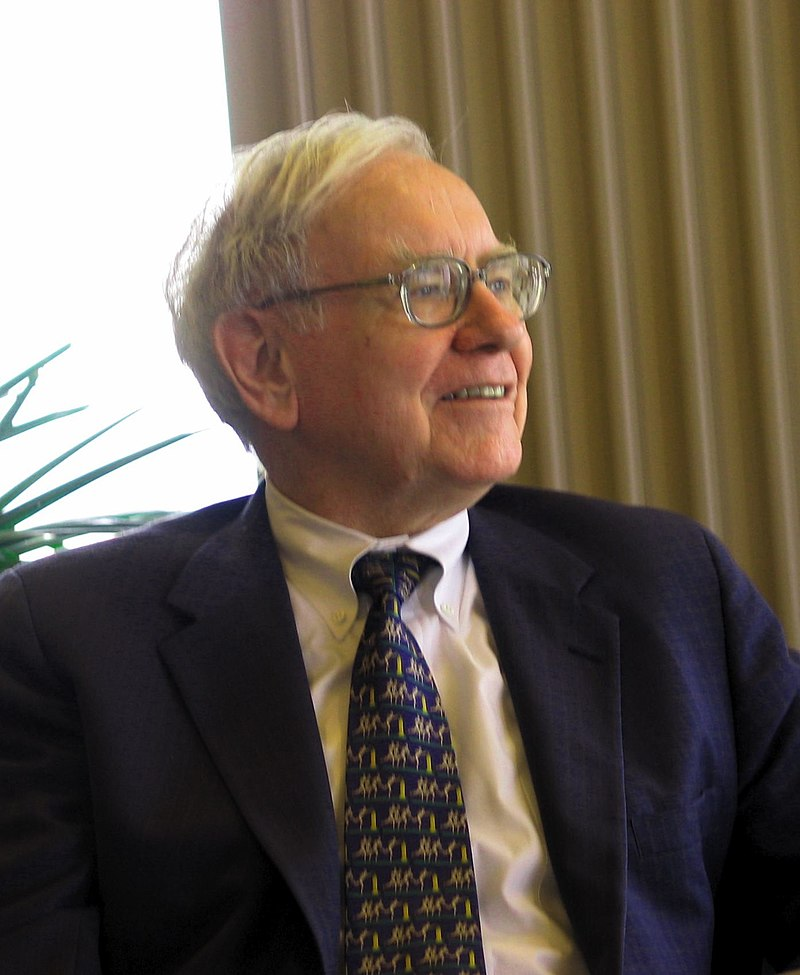
\includegraphics[width=1.5in]{WarrenBuffett}\\{\tiny\color{gray} CC BY-SA 2.0, Mark Hirschey}}
In the 1930s and 1940s, a young boy in Omaha, Nebraska spent nearly every spare hour in some entrepreneurial pursuit or another, ranging from delivering newspapers to purchasing and installing used pinball machines.  This single-minded focus on business meant that by the time he finished college, he had saved the equivalent of over \$100,000 in modern terms.

This boy, Warren Buffett, certainly benefited from some privileges, such as having the time to work and being able to keep everything he earned, but it is undeniable that his work ethic was impressive.  He didn't stop with those savings, though; through long-term investment, he parlayed those funds into one of the largest fortunes in the world (at the time of writing, Warren Buffett is the fourth-richest person in the world).  The ``Oracle of Omaha,'' who still lives in the home that he bought in 1957 for \$31,500, has pledged to give away 99\% of his vast fortune to charity.

Why do we begin with this story?  There are many other investors who were not so fortunate, but Warren Buffett is a dramatic example of the old adage, ``It takes money to make money.''  One of the most notable things about Buffett is his frugality; rather than spending his money, he has spent decades re-investing it.  Perhaps we could rephrase the adage in a slightly less pithy way:
\begin{center}
Money is expected to grow over time.
\end{center}

Take a look, for instance, at a graph of the Dow Jones Industrial Average over the past 30 years.  The DJIA is a value calculated by adjusting the sum of the prices of the stocks for thirty major companies such as Coca-Cola, Nike, Microsoft, and Walmart.  It can be used to give a quick snapshot of how the stock market in general is behaving.
\begin{center}
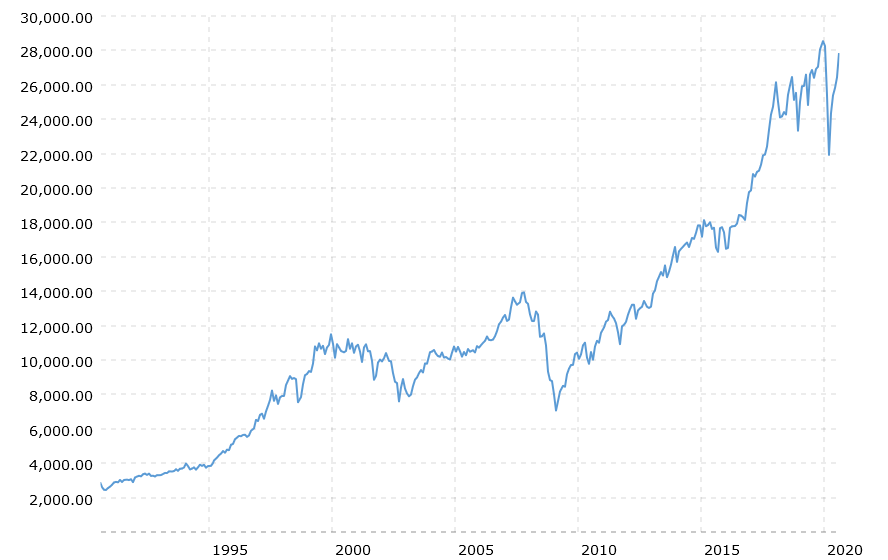
\includegraphics[width=0.8\textwidth]{DowJones}\\
\text{} \hfill {\color{gray} Source: Macrotrends.net}
\end{center}

The value of the Dow Jones index is fairly volatile, and there are notable dips (notice the big drop in 2007, when the Great Recession began, and how the graph began to creep up again in 2009, as the recession eased).  However, the overall trend is unmistakable: if you zoom out, the value of the stock market has increased steadily, and is expected to continue growing, even if there are short-term drops.

\subsection{Time Value of Money}
Let's take a smaller-scale example.  Suppose you want to start a small business; let's say for the sake of argument that you'll be starting a landscaping company.  You immediately run into a problem, though: if you had all the equipment you needed, you'd be able to start making money right away by offering your services.  However, you don't have everything you need.  You'll need a truck and a trailer, mowers and other equipment, and some form of advertising (business cards, signs, a website, etc.).  What you've run into is that same principle: ``It takes money to make money.''  If you had the money to start your business, you could invest in your landscaping company and use that to make more money.

So what do you do?  The solution is to go to a bank and take out a small-business loan, because the bank has the cash on hand, and they recognize that if they loan it to you, you'll be able to---through your hard work---multiply that money several times over, so you'll be able to repay them.

This is the foundation of the principle that we expect money to grow over time.  If you have some money today beyond what you need to cover living expenses, you can find some way to use it---either by adding your own hard work to it or finding somebody else who can do that---and by using it wisely, you can receive back more than you put in.

\begin{formula}{Time Value of Money}
\begin{center}
\marginnote{``Money is of the prolific, generating nature.  Money can beget money, and its offspring can beget more, and so on.''\\
\text{} \hfill -Benjamin Franklin}
Money is expected to grow over time.
\end{center}
We'll have specific formulas for this later, but for now, all we need is the basic principle.  For instance, \$100 today may be expected to be worth \$110 a year from now.  In this example, the \textbf{present value} is \$100, and the \textbf{future value} is \$110.
\end{formula}

Since this is the basis of the entire economy, we can simplify the big picture by envisioning money as something that grows.  There are many implications of this, but the most significant one is this: there is value to holding money right now.  Because of that, if you want to borrow money, you not only have to pay it back at some point, but you also have to pay extra on top of that for the privilege of holding onto the money for some time--this brings us to the crucial concept of \textbf{interest}.

Think back to the example of the landscaping company: you go to the bank and take out a small-business loan.  When you do, they will lay out the terms of the loan.  For instance, say you take out a loan of \$100,000 for 10 years.  That means that by the end of the 10 years, you'll have to pay back all of the original \$100,000, plus whatever interest the bank adds on top.  The question of \textbf{how} you pay it back, whether in one lump sum at the end or in smaller regular payments, will be addressed in later sections of this chapter.

\begin{formula}{Loans}
Here are a few terms that will be used frequently throughout the chapter:
\begin{itemize}
\item \textbf{Principal}: The amount of money borrowed
\item \textbf{Interest}: The fee added to the principal, which must also be paid
\item \textbf{Life of the loan}: The amount of time until the loan must be paid off
\end{itemize}
\end{formula}

In the example above, the principal is \$100,000 and the life of the loan is 10 years.\\

What about the interest?

\subsection{Interest Rates}
We need a fair way to decide how much interest to charge for a particular loan.  Let's start with a simple example.

Pretend that you are in the bank's position: you have money to loan out, and you're accepting loan applications.  Two people send in applications:
\begin{itemize}
\item One requests \$100,000 to buy a foreclosed house, fix it up, and resell it
\item The other requests \$500,000 to buy 5 foreclosed houses, fix them all up, and resell them
\end{itemize}
How much do you charge them in interest?

Clearly it wouldn't make sense to charge a flat rate.  Since both are making the same investment, but the second person is doing five times as much as the first, it's reasonable to assume that they will also see about five times the return as the first person.

Therefore, \textbf{interest scales with the amount of the loan}.  This means that interest is always a fraction of the principal, although interest rates are described using percentages.

\begin{formula}{Interest Rates}
Interest is always defined as a percentage of the principal.
\end{formula}

For instance, if you take out a loan of \$100 for a year and agree to pay 5\% interest, that means that at the end of the year you will owe \$100 plus 5\% of \$100.

This means that we need to be comfortable working with percentages before we can solve the problems later in this chapter.  Because of this, we'll include a short discussion of percentages here.  More examples can be found in the review chapter included at the end of the book, and the next section will cover applied problems that use percentages.

\subsection{Percentages}
\marginnote{\textbf{Percent:} \\ number of hundredths}
A percentage is simply another way to represent a fraction or a decimal.  The word ``percent'' means ``per 100,'' or ``number of hundredths.''

\begin{proc}{Percents, Fractions, and Decimals}
Since percent (\%) means ``number of hundredths,'' we can convert decimals to percents by multiplying by 100 (or moving the decimal point two places to the right).\\

We can convert fractions to percents the same way by first writing them as decimals.
\end{proc}

\begin{example}[https://www.youtube.com/watch?v=UZHLvEmFrOk&list=PLfmpjsIzhztsZtnb7HnXrQ8SLoiOCIcAM&index=1]{Converting to Percentages}
Convert each of the following to a percentage:\\

\begin{tabular}{l l l}
(a) $\dfrac{2}{5}$ & (b) $0.15$ & (c) $\dfrac{9}{2}$
\end{tabular}

\sol
\begin{center}
\begin{tabular}{l l l}
(a) $\dfrac{2}{5} = 0.40 = 40\%$ & (b) $0.15 = 15\%$ & (c) $\dfrac{9}{2} = 4.50 = 450\%$
\end{tabular}
\end{center}
\end{example}

\begin{try}[http://hartleymath.com/versatilemath/tryit/\#/financial-mathematics--converting-to-percentages]
Convert each of the following to a percentage:\\

\begin{tabular}{l l l}
(a) $\dfrac{3}{5}$ & (b) $0.7$ & (c) 2
\end{tabular}
\end{try}

This process can be reversed to convert a percentage to a decimal, which we'll want to do frequently in later sections of this chapter.

To do so, simply remove the percent symbol and divide the percentage by 100 (i.e. move the decimal point two places to the left).
%\vfill
%\pagebreak

\begin{example}[https://www.youtube.com/watch?v=d770dB9RHIc&list=PLfmpjsIzhztsZtnb7HnXrQ8SLoiOCIcAM&index=2]{Converting Percents to Decimals}
Convert the following percentages to decimals:\\

\begin{tabular}{l l l}
(a) 28\% & (b) 104\% & (c) 0.37\%
\end{tabular}

\sol
\begin{center}
\begin{tabular}{l l l}
(a) $28\% = 0.28$ & (b) $104\% = 1.04$ & (c) $0.37\% = 0.0037$
\end{tabular}
\end{center}
\end{example}
\pagebreak

\subsection{What's Coming Next}
With that, we're ready to dive into the rest of the chapter and explore all kinds of financial concepts.  The most important principle that you need to carry with you is the simple idea we've seen several times: money is expected to grow over time, so whenever someone borrows money, the lender expects to not only get the principal back, but also some percentage in interest.  The same concept applies when you put money into a bank account or other investment: you can expect to receive interest as payment for that account holding your money.

Here's what to expect in the rest of the chapter:
\paragraph{Section 1.2: Applied Percentage Problems} Solve word problems that involve percentages, like ``If a \$20 shirt is discounted by 15\%, what's the sale price?''

\paragraph{Section 1.3: Simple and Compound Interest} Learn about compound interest and how it makes investments grow with incredible speed.

\paragraph{Section 1.4: Saving for Retirement} It may seem far away now, but if you learn nothing else from this chapter, remember this: start saving for retirement \textbf{now}, even if you can only afford to save a little at a time.

\paragraph{Section 1.5: Mortgages and Credit Cards} Car payments, home mortgages, and credit cards are all examples of \textit{installment loans}, which are paid back with regular payments.

\paragraph{Section 1.6: Income Tax} The endlessly quotable Benjamin Franklin famously said, ``In this world nothing can be said to be certain, except death and taxes.''  Learn the basics of how income tax is calculated.